\documentclass[a4paper,11pt]{article}
\usepackage[utf8]{inputenc}
\usepackage[T1]{fontenc}
\usepackage[french]{babel}
\usepackage{textcomp}
\usepackage{listings}
\usepackage{pdfpages}
\usepackage{array}
\usepackage{titling}
\usepackage{geometry}

\geometry{hmargin=2.5cm,vmargin=1.5cm}
\setlength{\hoffset}{-18pt}        
\setlength{\oddsidemargin}{0pt} % Marge gauche sur pages impaires
\setlength{\evensidemargin}{9pt} % Marge gauche sur pages paires
\setlength{\marginparwidth}{54pt} % Largeur de note dans la marge
\setlength{\textwidth}{481pt} % Largeur de la zone de texte (17cm)
\setlength{\marginparsep}{2pt} % Séparation de la marge
\setlength{\topmargin}{0pt} % Pas de marge en haut
\setlength{\headheight}{10pt} % Haut de page
\setlength{\headsep}{10pt} % Entre le haut de page et le texte
\setlength{\footskip}{27pt} % Bas de page + séparation
\setlength{\textheight}{708pt} % Hauteur de la zone de texte (25cm)

\setlength{\droptitle}{-4cm}
\title{Synthèse - Machine Learning}
\author{Léa Calem - Fatima Layla - Laureline Martin}

\begin{document}

\maketitle
	
\section{Description du jeu de données}
	\subsection{Les données}
	% \subsubsection{Modélisation des données sous forme de matrice}
		Nous disposons de 14 000 images représentant soit des t-shirts/tops, soit des robes. La classe $C_1 =$ \{0 T-shirt/top\} et la classe $C_2 =$ \{3 Dress\}.
		\begin{itemize}
			\item 7 000 images de la classe $C_1$
			\item 7 000 images de la classe $C_2$
		\end{itemize}
		Les images de taille 28x28 pixels (784 pixels) composées de niveau de gris (valeur allant de 0 à 255). Sur ces images, seul l’objet est coloré donc le reste de l’image est en blanc, la valeur des pixels à 0.\\
		Ces images sont issues des classes 0 et 3 du jeu données Fashion-MNIST (http://www.openml.org/d/40996). 
	\subsection{Séparation des jeux de données}
		\begin{enumerate}
			\item Données d’entraînement : sous-ensemble de données destiné à l’apprentissage du modèle. Nous utilisons 75\% des données pour l'apprentissage, soit 10 500 images.
			\item Données de test : sous-ensemble de données destiné à l’évaluation du modèle (ce jeu de données ne doit en aucun cas être utilisé lors de la conception du modèle). Nous utilisons 25\% des données, soit 3 500 images.
		\end{enumerate}

	\subsection{Description statistique}
		Ci-dessous, un graphe représentant le nombre de pixels différents de 0 en fonction de la classe.
		Nous avons divisé l’image en 3 tiers horizontaux, puis nous calculons la moyenne du blanc de la 1ère et 3éme partie. Les t-shirts ont une moyenne de blanc moins importante sur le 1er tiers de l'image que sur le 3e tiers (car les manches sont plus larges que le reste du tissu), tandis que les moyennes de blanc pour les robes sont similaires pour le 1er et le 3e tiers de l'image (manches et la jupe du vêtement prennent autant d'espace sur l'image).\\
		%images
		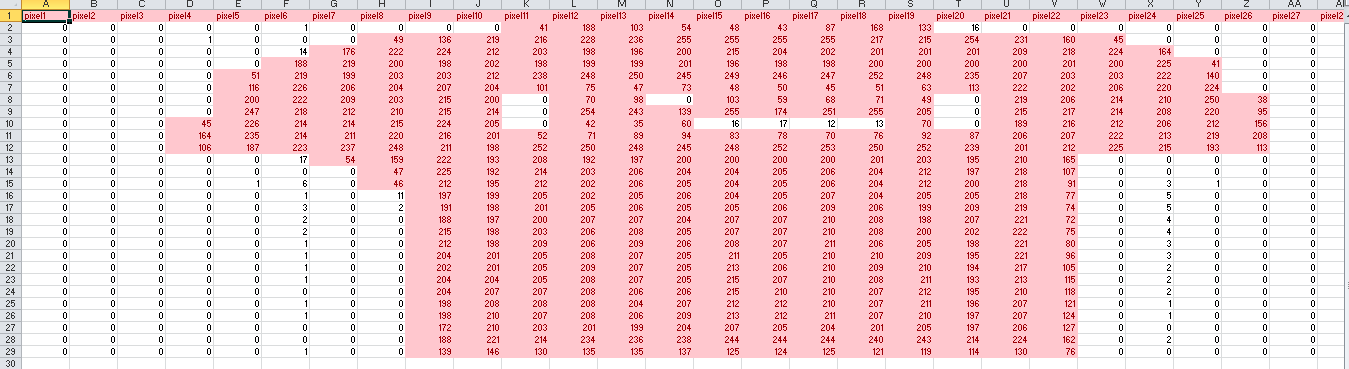
\includegraphics[scale = 0.25]{fichiers/ex_tshirt.PNG}
		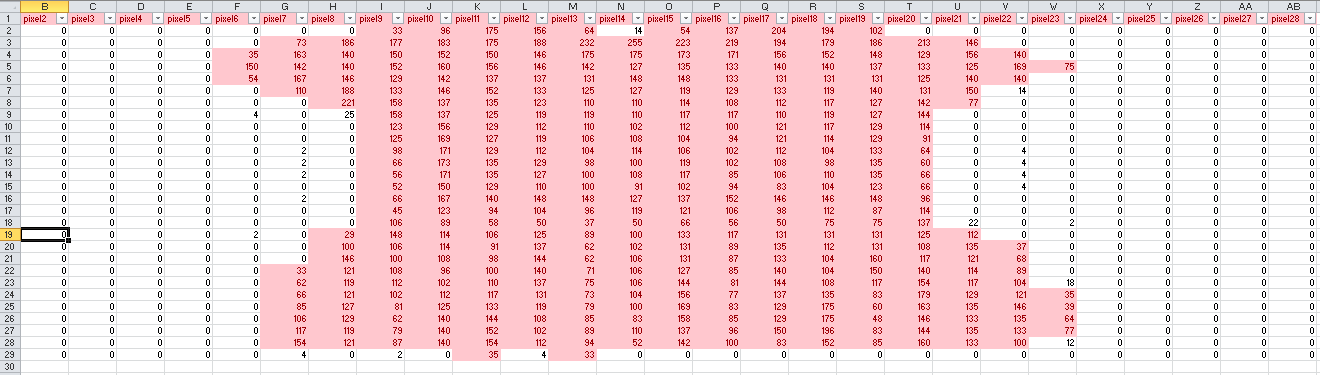
\includegraphics[scale = 0.25]{fichiers/ex_robe.PNG}\\
		\\
		\vfill\begin{center} 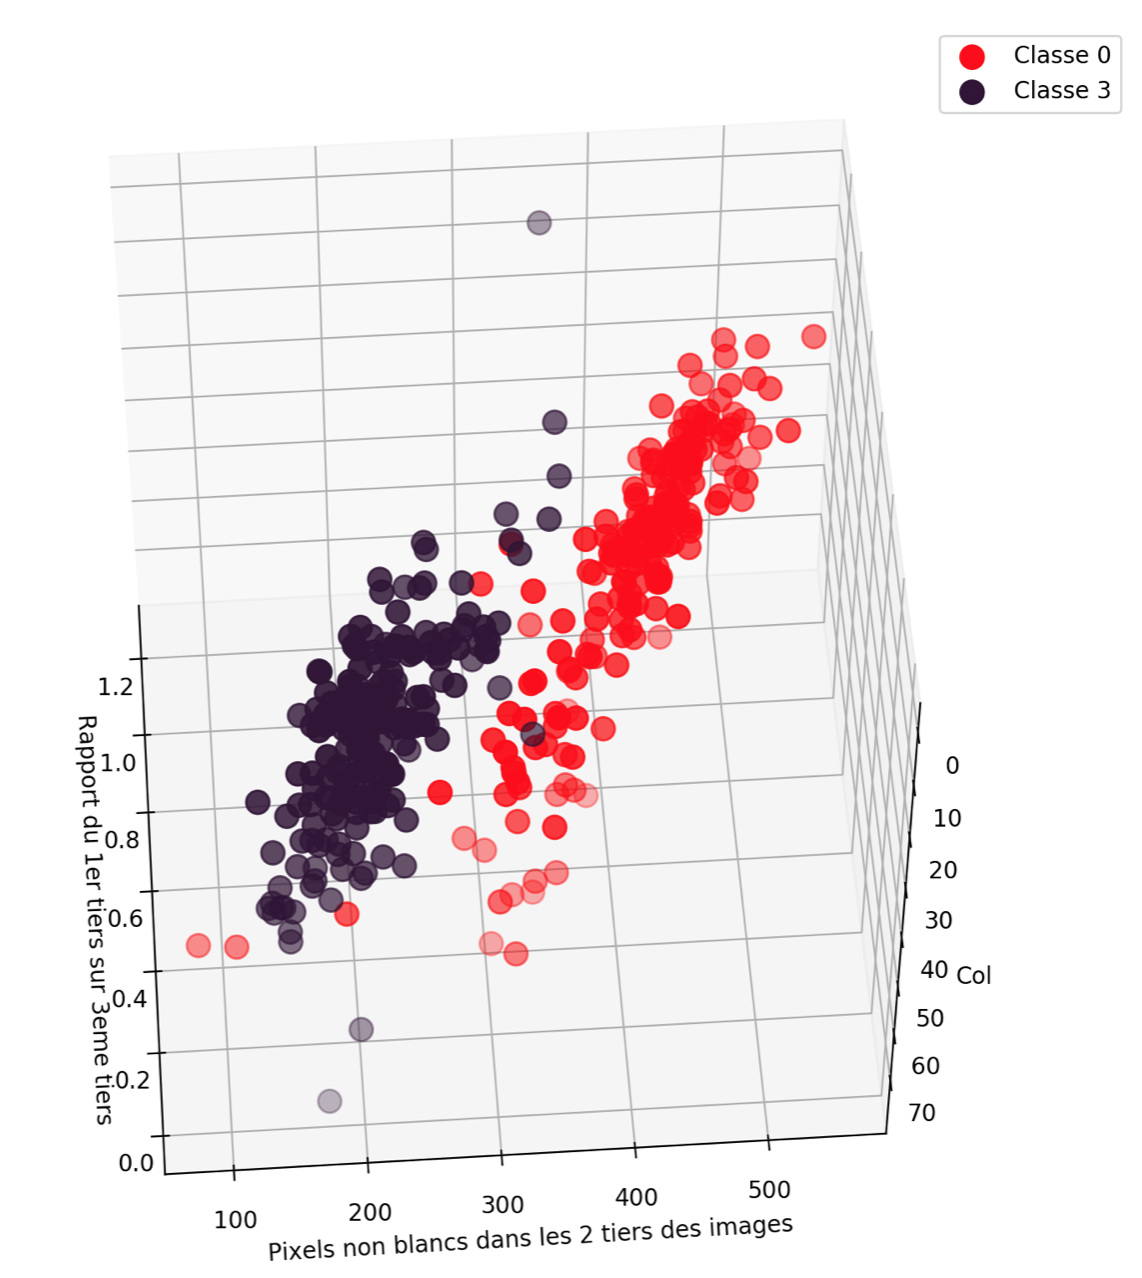
\includegraphics[scale = 0.6]{fichiers/rapport.PNG} \end{center}\vfill
		


\newpage
\section{Méthodologie}
	\subsection{Méthodologie générale}
		Dans ce projet, nous allons classifier des images en deux catégories : t-shirts/tops ou robes.\\
		Les méthodes d'apprentissages que nous allons utiliser sont de type supervisées car nos données sont déjà annotées :
		$$ S = {(x_i, y_i)} $$
		Tel que : $x_i$ = ième image de l'ensemble des images, $y_i$ = ième étiquette de l'ensemble des étiquettes des classes $C_1$ et $C_2$.\\
		% Classification : $y_i = {C_1, C_2}$.
		Avec les classes : $C_1 =$ \{0 T-shirt/top\} et $C_2 =$ \{3 Dress\}.\\
		\\
		Nous allons utiliser plusieurs méthodes d’apprentissage qui vont nous permettre de définir la fonction d'appprentissage $h(x)$ telle que : $h(x) = (\hat y)$. Ainsi, nous obtiendrons des valeurs $(\hat y)_i$ proches des $y_i$, pour tout $(x_i, y_i)$ appartenant à $S$.\\
		%(cours 02\_methodo\_etu.pdf/ slide 9)

	\subsection{Paramètres}
		Comme les images $x_i$ sont bruitées, nous supposons que les pixels ayant une valeur < 25 sont blanc.\\
		Nous évaluons comme paramètre l'écart entre blanc et gris tous les 28 pixels.

	\subsection{Méthodes d'apprentissage utilisées}
		\begin{itemize}
			\item Les K-NN (K plus proches voisins) : Fatima
			\item La régression : Lauréline
			\item SVM : Léa
		\end{itemize}

	\subsection{Protocole de comparaison}
		Pour comparer les résultats des différentes méthodes d'apprentissages utilisées, nous évaluons le taux d’erreurs sur des jeux identiques de données.


\end{document}